\documentclass[landscape]{article}
\usepackage[paperwidth=292mm, paperheight=123mm, margin=0cm]{geometry}
\usepackage{tikz}
\usepackage{xcolor}
\definecolor{myBlue}{RGB}{173, 216, 230}
\definecolor{myGrey}{RGB}{200, 200, 200}
\usetikzlibrary{positioning, shapes.geometric, arrows}

% Define styles
\tikzstyle{node} = [rectangle, rounded corners, minimum width=1.5cm, minimum height=1cm, text centered, draw=black]
\tikzstyle{arrow} = [thick,->,>=stealth]

\begin{document}

\begin{figure}[h]
    \centering
    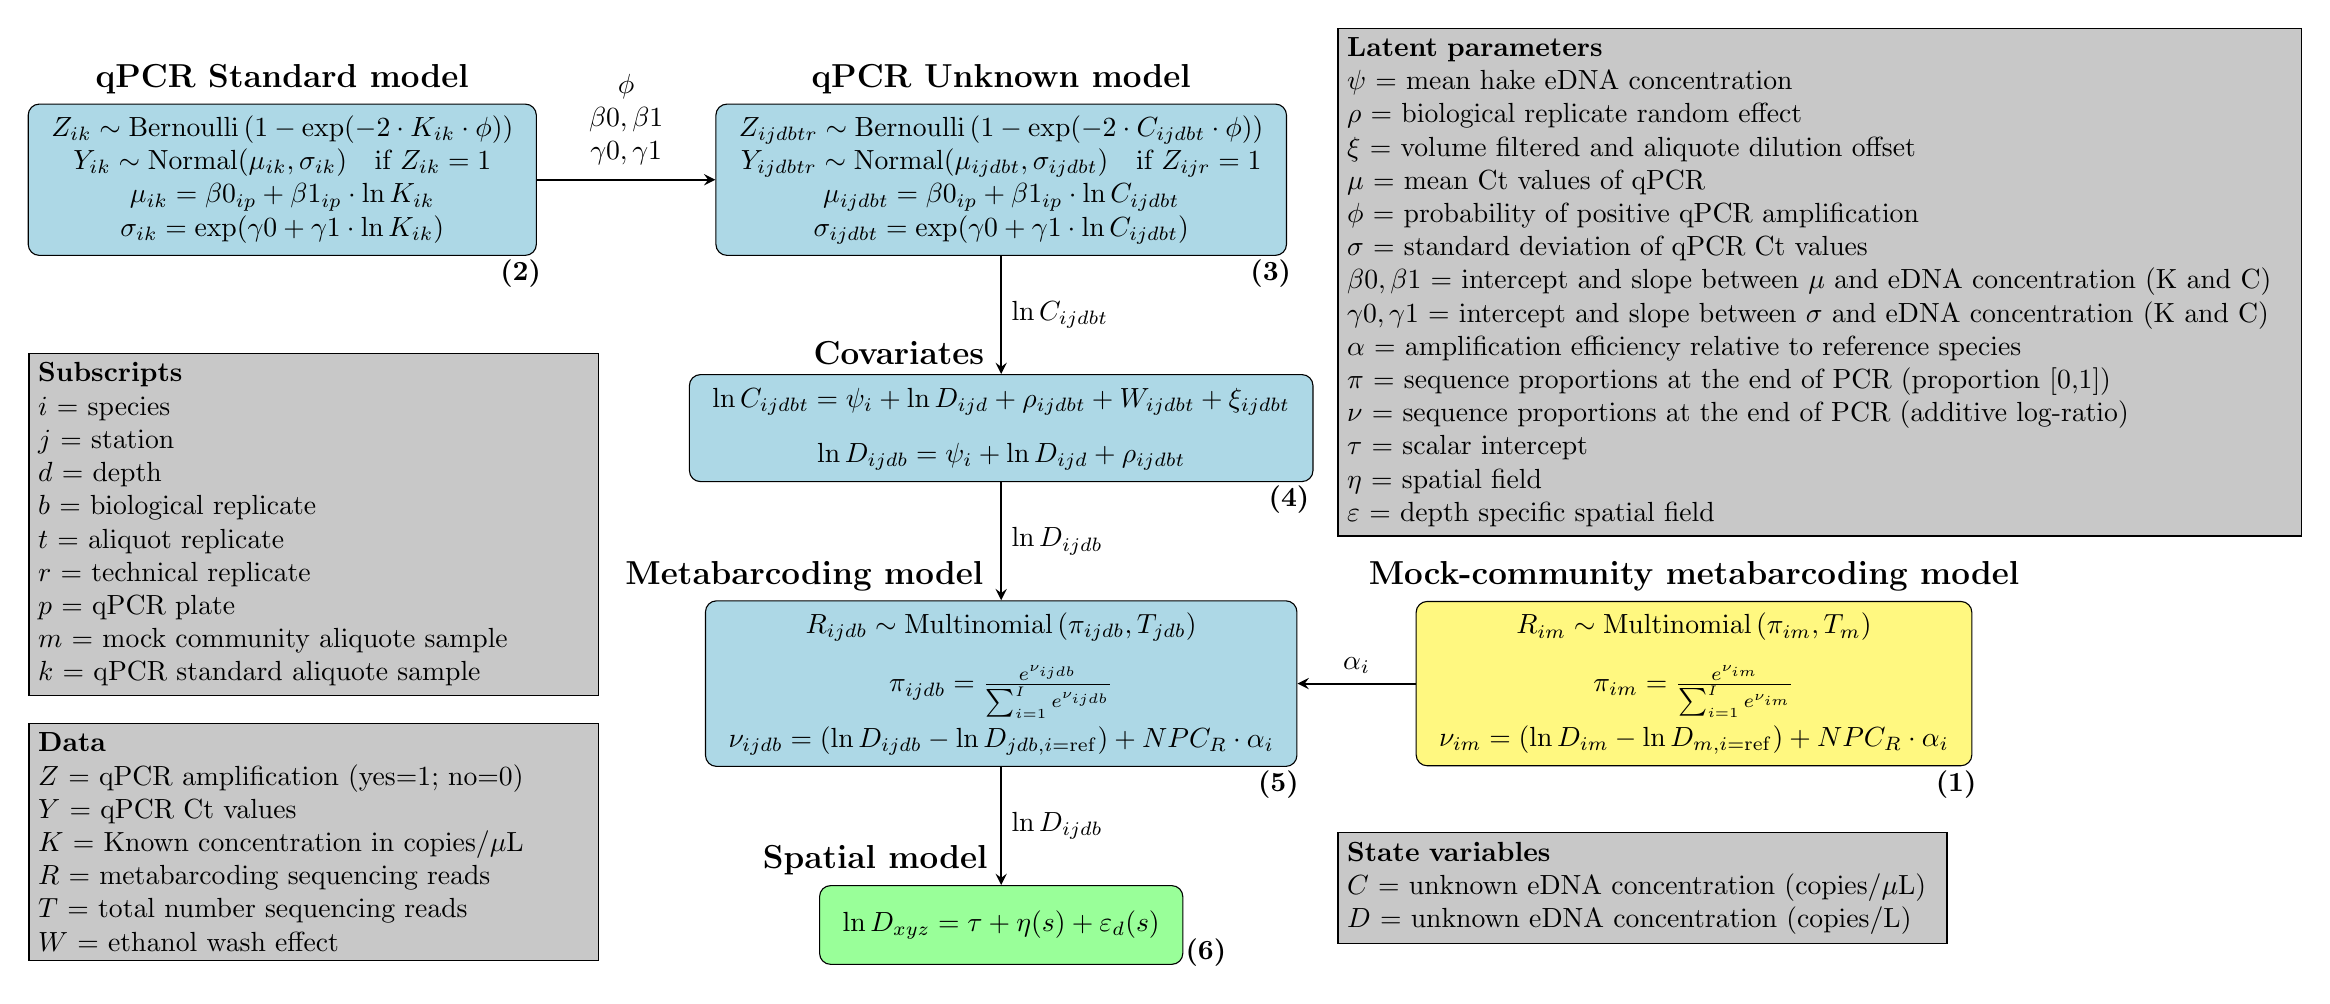
\begin{tikzpicture}[node distance=1.5cm]
        % Nodes
\node (qPCR_st) [node, fill=myBlue] at (0,0) {
    $\begin{array}{c}
        Z_{ik} \sim \mathrm{Bernoulli} \left( 1 - \exp(-2 \cdot K_{ik} \cdot \phi) \right) \\
        Y_{ik} \sim \mathrm{Normal} (\mu_{ik}, \sigma_{ik}) \quad \textnormal{if } Z_{ik} = 1 \\
        \mu_{ik} = \beta0_{ip} + \beta1_{ip} \cdot \ln K_{ik} \\
        \sigma_{ik} = \exp(\gamma0 + \gamma1 \cdot \ln K_{ik})
    \end{array}$
};

\node [above=of qPCR_st, yshift=-1.5cm, font=\large\bfseries] {qPCR Standard model};
\node[anchor=south east] at ([xshift=5pt, yshift=-15pt] qPCR_st.south east) {\textbf{(2)}};


\node (qPCR_en) [node, right=of qPCR_st, fill=myBlue]  at (4,0) {
    $\begin{array}{c}
        Z_{ijdbtr} \sim \mathrm{Bernoulli} \left( 1 - \exp(-2 \cdot C_{ijdbt} \cdot \phi) \right) \\
        Y_{ijdbtr} \sim \mathrm{Normal} (\mu_{ijdbt}, \sigma_{ijdbt}) \quad \textnormal{if } Z_{ijr} = 1 \\
        \mu_{ijdbt} = \beta0_{ip} + \beta1_{ip} \cdot \ln C_{ijdbt} \\
        \sigma_{ijdbt} = \exp(\gamma0 + \gamma1 \cdot \ln C_{ijdbt})
    \end{array}$
};
\node [above=of qPCR_en, yshift=-1.5cm, font=\large\bfseries] {qPCR Unknown model};
\node[anchor=south east] at ([xshift=5pt, yshift=-15pt] qPCR_en.south east) {\textbf{(3)}};


\node (covariates) [node, below=of qPCR_en, fill=myBlue] { 
% + \delta0_{ijdbt} \cdot
% + \delta1_{ijdb}
    $\begin{array}{c}
        %\ln C_{ijdbt} = \psi_i + \ln D_{ijd} + \rho_{ijdbt} + \omega_{ijdbt} + \xi_{ijdbt} \\[8pt]
        \ln C_{ijdbt} = \psi_i + \ln D_{ijd} + \rho_{ijdbt} + W_{ijdbt} + \xi_{ijdbt} \\[8pt]
        \ln D_{ijdb} = \psi_i + \ln D_{ijd} + \rho_{ijdbt}
    \end{array}$
};
\node [above=of covariates, yshift=-1.5cm, xshift=-1.3cm, font=\large\bfseries] {Covariates};
\node[anchor=south east] at ([xshift=2pt, yshift=-15pt] covariates.south east) {\textbf{(4)}};


\node (metabarcoding) [node, below=of covariates, fill=myBlue] {
    $\begin{array}{c}
        R_{ijdb} \sim \mathrm{Multinomial} \left( \pi_{ijdb}, T_{jdb} \right) \\[8pt]
        \pi_{ijdb} = \frac{e^{\nu_{ijdb}}}{\sum_{i=1}^{I} e^{\nu_{ijdb}}} \\[8pt]
        \nu_{ijdb} = (\ln D_{ijdb} - \ln D_{jdb, i=\mathrm{ref}}) + NPC_{R} \cdot \alpha_i
    \end{array}$
};
\node [above=of metabarcoding, yshift=-1.5cm, xshift=-2.5cm, font=\large\bfseries] {Metabarcoding model};
\node[anchor=south east] at ([xshift=4pt, yshift=-15pt] metabarcoding.south east) {\textbf{(5)}};


\node (mock) [node, right=of metabarcoding, fill=yellow!50] {
    $\begin{array}{c}
        R_{im} \sim \mathrm{Multinomial} \left( \pi_{im}, T_{m} \right) \\[8pt]
        \pi_{im} = \frac{e^{\nu_{im}}}{\sum_{i=1}^{I} e^{\nu_{im}}} \\[8pt]
        \nu_{im} = (\ln D_{im} - \ln D_{m, i=\mathrm{ref}}) + NPC_{R} \cdot \alpha_i
    \end{array}$
};
\node [above=of mock, yshift=-1.5cm, font=\large\bfseries] {Mock-community metabarcoding model};
\node[anchor=south east] at ([xshift=5pt, yshift=-15pt] mock.south east) {\textbf{(1)}};


\node (spatial) [node, below=of metabarcoding, fill=green!40] {
    $\begin{array}{c}
        \ln D_{xyz} = \tau + \eta(s) + \varepsilon_{d}(s)
    \end{array}$
};
\node [above=of spatial, yshift=-1.5cm, xshift=-1.6cm, font=\large\bfseries] {Spatial model};
\node[anchor=south east] at ([xshift=19pt, yshift=-4pt] spatial.south east) {\textbf{(6)}};



        % Arrows
        \draw [arrow] (qPCR_st) -- node[midway, above] {
        $\begin{array}{c}
            \phi \\ \beta0, \beta1 \\ \gamma0, \gamma1
        \end{array}$} (qPCR_en);
        \draw [arrow] (qPCR_en) -- node[midway, right] {$\ln C_{ijdbt}$} (covariates);
        \draw [arrow] (covariates) -- node[midway, right] {$\ln D_{ijdb}$} (metabarcoding);
        \draw [arrow] (mock) -- node[midway, above] {$\alpha_i$} (metabarcoding);
        \draw [arrow] (metabarcoding) -- node[midway, right] {$\ln D_{ijdb}$} (spatial);

% Legend: Latent Parameters
\node (parameters) [rectangle, draw, align=left, right=of qPCR_en, text width=12cm, fill=myGrey] at (11.9,-1.3){
    \textbf{Latent parameters} \\
    $\psi$ = mean hake eDNA concentration \\
    %$\delta0, \delta1$ = offset from mean hake \\
    $\rho$ = biological replicate random effect \\
    %$\omega$ = ethanol wash effect \\
    $\xi$ = volume filtered and aliquote dilution offset \\
    $\mu$ = mean Ct values of qPCR \\
    $\phi$ = probability of positive qPCR amplification \\
    $\sigma$ = standard deviation of qPCR Ct values \\
    $\beta0, \beta1$ = intercept and slope between $\mu$ and eDNA concentration (K and C) \\
    $\gamma0, \gamma1$ = intercept and slope between $\sigma$ and eDNA concentration (K and C) \\
    $\alpha$ = amplification efficiency relative to reference species \\
    $\pi$ = sequence proportions at the end of PCR (proportion [0,1]) \\
    $\nu$ = sequence proportions at the end of PCR (additive log-ratio)\\
    $\tau$ = scalar intercept\\
    $\eta$ = spatial field \\
    $\varepsilon$ =  depth specific spatial field
};

% Legend: Subscripts
\node (subscripts) [rectangle, draw, align=left, below=of qPCR_st, text width=7cm, fill=myGrey] at (0.4,-0.7) {
    \textbf{Subscripts} \\
    $i$ = species \\
    $j$ = station \\
    $d$ = depth \\
    $b$ = biological replicate \\
    $t$ = aliquot replicate \\
    $r$ = technical replicate \\
    $p$ = qPCR plate \\
    $m$ = mock community aliquote sample \\
    $k$ = qPCR standard aliquote sample
};
% Legend: Data
\node (data) [rectangle, draw, align=left, below=of subscripts, text width=7cm, fill=myGrey] at (0.4,-5.4){
    \textbf{Data} \\
    $Z$ = qPCR amplification (yes=1; no=0) \\
    $Y$ = qPCR Ct values \\
    $K$ = Known concentration in copies/$\mu$L \\
    $R$ = metabarcoding sequencing reads \\
    $T$ = total number sequencing reads \\
    $W$ = ethanol wash effect
};
% Legend: State variables
\node (state) [rectangle, draw, align=left, right=of qPCR_en, text width=7.5cm, fill=myGrey] at (11.9,-9){
    \textbf{State variables} \\
    $C$ = unknown eDNA concentration (copies/$\mu$L) \\
    $D$ = unknown eDNA concentration (copies/L)
};
    \end{tikzpicture}
    %\caption{Multifish DAG}
\end{figure}

\end{document}